\chapter{Evaluation of Inductive Model Synthesis\label{chapter:evaluation}}

This chapter reports the results obtained when evaluating our inductive LTS synthesis technique from Chapter~\ref{chapter:inductive-synthesis}. Section \ref{section:evaluation-objectives-and-approach} discusses our evaluation objectives and gives an overview of the chosen approach. Section \ref{section:evaluation-experiments-on-case-studies} presents the results of evaluating our algorithms on three case-studies. These evaluations are complemented by experiments conducted on synthetic datasets, whose setup and results are presented in Section \ref{section:evaluation-experiments-on-synthetic-data}. Our main conclusions are drawn in Section \ref{section:evaluation-summary}.

\section{Objectives and approach\label{section:evaluation-objectives-and-approach}}

The aim of this chapter is to evaluate our inductive synthesis technique in the light of the thesis objectives. The idea is to check whether our synthesis approach provides an effective way of exploring requirements and conducting system design. Or, in terms of the requirements discussed in Chapter~\ref{chap:introduction},

\begin{quotation}
\emph{How well does it help building \emph{adequate}, \emph{complete}, \emph{consistent} and \emph{precise} models for the target system considered?}
\end{quotation}

Such a question is difficult to answer in absolute terms. Answers can however be provided in two ways:
\begin{enumerate}
\item[a)] By comparing the technique with existing ones, either theoretically or on common benchmarks.
\item[b)] By using the technique in controlled experiments. Here, controlled parameters provide variation points to conduct comparisons.
\end{enumerate}
This chapter focusses on the second way of conducting evaluation. A discussion of how our inductive synthesis approach compares and integrates with existing techniques can be found in Chapter~\ref{chapter:related-work}, thereby completing the evaluation given here.

When our inductive synthesis technique is considered in isolation, the question of how well it performs can already be partially answered. For instance, our technique builds \emph{consistent} models by construction; by design, it also helps \emph{completing} them through scenario questions. However, other related questions cannot be answered so simply:
\begin{itemize}
\item How adequate are the synthesized state machines? 
\item What is the impact of fluent, goal and domain knowledge injection on model adequacy?
\item Is the approach usable by end-users? 
\item How many iterations are needed to obtain models considered complete?
\item Does the inductive technique scales and stays usable on large systems?
\end{itemize}

Controlled experiments have thus been conducted to provide answers to those questions. In practice, two kinds of evaluation have been considered, as reflected by the following sections. The specific evaluation protocols used will be described in each case.
\begin{itemize}

\item Section \ref{section:evaluation-experiments-on-case-studies} discusses evaluations conducted on three case studies involving multiple models. The aim here is to evaluate the feasibility of inductive LTS synthesis in practice. Our ISIS tool presented in Section \ref{section:tool-support-isis} has been used as an effective support for designing and conducting the evaluations described there.

\item Section \ref{section:evaluation-experiments-on-synthetic-data} complements this case-driven evaluation with experiments conducted on random automata and samples. The aim here is to study the performance of QSM and ASM in a more systematic way using synthetic datasets whose size grows significantly beyond the average one of the case studies. This will also allow us to compare our techniques with state-of-the-art induction algorithms. To achieve sound comparisons, our evaluation protocol inspires from a benchmark known as Abbadingo \cite{Lang:1998} (see Section~\ref{subsection:evaluation-synthetic-protocol}).
\end{itemize}

Using the ISIS tool on case-studies provides a first evaluation \emph{in situ}. The overall effectiveness of our multi-view synthesis approach will be illustrated on a typical run. In addition, controlled parameters of the experiments provide comparison points to answer finer-grained evaluation questions. Those controlled parameters are:
\begin{itemize}
\item The size the target system LTS, either because a selected case-study or controlled by a random generation procedure.
\item The heuristics used for state merging: the RPNI search order or the Blue-fringe optimization.
\item The presence of absence of an oracle answering scenario questions.
\item The number of fluents and goals injected to prune the induction process.
\item The use of control information in scenarios and the richness of such knowledge.
\end{itemize}

Three measures have been collected when conducting the various experiments. Those measures have a clear impact on the adequacy and usability of the synthesis technique. Therefore, they allow making the link between the controlled parameters and answers to our evaluation questions.
\begin{description}
\item[Model adequacy] Roughly speaking, \emph{model adequacy} captures \emph{how well} an inferred model matches the expected target behavior model. 

Model adequacy is easy to measure in controlled experiments in which, by design, the target model is then known. Depending on the experiment, we will use either a binary value or a finer-grained one.
\begin{itemize}
\item In the former case, the adequacy measure simply captures whether the learned model is \emph{the same} as the target model or not, in terms of behavioral equivalence (see Definition~\ref{definition:trace-equivalence}).
\item In the latter case, an \emph{accuracy} measure will be used; such measure will range from 0.0 to 1.0 dependent on whether the learned model is considered far or close to the target model. This will be estimated through test samples (see Section~\ref{subsection:evaluation-synthetic-protocol}).
\end{itemize}
Note that adequacy is harder to assess on real-world case studies where the target model is unknown. In practice, human inspection of the learned models is required.

\item[Number of scenario questions] The number of queries generated to the oracle is a key measure for the usability of QSM in practice. 

This is certainly true when the oracle is a human being. A large number of queries might also be a problem with automated oracles; online oracles may be slow, others might be expensive, etc.

\item[Induction time] The time taken to infer a model deserves special attention. While a reasonable induction time is desirable in any case, fast, real-time interactions are required for usability of QSM by a human oracle.
\end{description}

Our experiments were designed to isolate the effect on the three measures above of the orthogonal features of our inductive technique. They quantify the gains and costs of the following ones in particular:
\begin{itemize}
\item The use of an oracle who can answer scenario questions: a gain is expected in model adequacy at the cost of a longer induction time.
\item The use of the Blue-fringe heuristic instead of the RPNI search order: a gain in adequacy is expected as well as a reduction of the number of scenario questions;
\item The use of domain knowledge such as fluent and goals: a gain in adequacy and a reduction of scenario questions should be observed as well;
\item The use of control information encoded into a hMSC: here also, a gain in adequacy is expected.
\end{itemize}


\section{Evaluations on case studies\label{section:evaluation-experiments-on-case-studies}}

QSM and ASM were evaluated on three different case studies of varying complexity. The first one is a mine pump system inspired from~\cite{Joseph:1996} and often used as a ``benchmark'' in the literature. The second case study refers to an extended version of the train system used here as a running example. The third one is a phone system handling communications between a caller and a callee.

\subsection{Evaluation methodology}

Beyond a practical evaluation of our tool-supported approach to multi-view LTS synthesis, our objective was to assess the impact of constraining induction through fluents, models of external components, domain descriptions and goals. Such impact was measured in terms of the number of generated scenario questions and the adequacy of the synthesized models. Induction time was also measured so as to check that fast interactions with the oracle are observed.

For each case study, we proceeded in two steps:
\begin{enumerate}
\item\label{stepA}
\begin{enumerate}
\item\label{CondA} Design a scenario collection allowing for meaningful subsequent comparison, that is, sufficiently rich to allow an adequate system LTS to be induced under one setting of the experiment at least (see hereafter).
\item\label{CondB} Define a common set of fluent definitions identifiable from this scenario collection. From this set of fluents, define a common set of domain properties and goals.
\end{enumerate}
\item\label{stepB} Evaluate the techniques on this scenario collection, without and then with fluents, goals, domain descriptions, or models of external components.
\end{enumerate}

In Step~\ref{stepA}, the richness condition on the scenario collection~(a) amounts to require the collection to be structurally complete; every transition in the target system LTS must occur in at least one scenario (see Section \ref{section:inductive-background}). The ISIS tool was used to incrementally set up such a scenario collection (see Section \ref{section:tool-support-isis}):
\begin{itemize}
\item An initial set of scenarios that end-users would typically provide was first selected.
\item By generating scenario questions, adding domain properties and goals, and validating the induced LTS, additional scenarios were found that were initially missing. 
\item Some of these scenarios were added to the collection for the comparisons in Step~\ref{stepB}. Added scenarios have been selected so as to reach a structurally complete collection of scenarios without making it too rich.
\end{itemize}

\begin{table}[H]
\centering
\begin{tabular}{|l||c|c|c||c|c|c|}\hline
Problem  & Events & States & Trans. & $|S^+|$ & $|S^-|$ & Avg. length\\\hline\hline
Mine Pump& 8      & 10     & 13          & 3     & 0     & 8\\\hline
Train    & 13     & 17     & 23          & 3     & 0     & 9\\\hline
Phone    & 16     & 23     & 33          & 6     & 4     & 11\\\hline
\end{tabular}
\caption{Sizes of the case studies.\label{CaseStudies}}
\end{table}

The size of the scenario collection resulting from Step~\ref{stepA} is shown in Table~\ref{CaseStudies}. $|S^+|$ and $|S^-|$ denote the number of positive and negative scenarios, respectively. The average scenario length is reported in the last column. The size of the target system LTS are also reported in terms of number of different event labels (alphabet size), states, and transitions. 

In order to measure the number of generated scenario questions in Step \ref{stepB}, an oracle was implemented to simulate the end-user. This oracle knows the system LTS for each problem and correctly classifies generated scenario as positive or negative. Note that this is a strong assumption on the oracle, especially when played by an end-user in practice; this issue has been discussed in Section~\ref{section:inductive-discussion}.

%%%%%

\subsection{RPNI search order vs. Blue-fringe strategy\label{subsection:evaluation-bluefringe-on-casestudies}}

Table~\ref{RPNI:Blue-fringe} reports the results obtained when running QSM with the RPNI search order and the Blue-fringe heuristics, respectively. In the sequel, these two settings will be denoted by QSM-rpni and QSM-fringe, respectively. The comparisons are made without additional knowledge to constrain induction. 

\begin{table}[H]
\centering
\begin{tabular}{|l||l||c|c|c|}\hline
Problem   & Algorithm   &$Q^+$&$Q^-$& Model adequacy\\\hline\hline
Mine Pump & QSM-rpni    & 1   & 30  & missing/unallowed traces\\\cline{2-5}
          & QSM-fringe  & 1   & 4   & adequate model\\\hline
Train     & QSM-rpni    & 4   & 83  & adequate model\\\cline{2-5}
          & QSM-fringe  & 5   & 5   & adequate model\\\hline
Phone     & QSM-rpni    & 5   & 171 & missing/unallowed traces\\\cline{2-5}
          & QSM-fringe  & 5   & 19  & missing/unallowed traces\\\hline
\end{tabular}
\caption{RPNI search order versus Blue-Fringe strategy for QSM.\label{RPNI:Blue-fringe}}
\end{table}

The table shows the number of queries the oracle had to answer together with a binary measure of model adequacy. $Q^+$ and $Q^-$ denote the number of accepted and rejected scenario questions, respectively. The model is said to be \emph{adequate} if it matches the known target LTS, formally if the two models are trace equivalent (see Definition \ref{definition:trace-equivalence}). 

The following main observations can be made from these results:
\begin{itemize}
\item The large number of generated questions makes QSM-rpni unusable with end-users on bigger systems. In contrast, the number of rejected scenario questions is drastically reduced thanks to the Blue-fringe search strategy. 
\item In the phone system, an adequate system LTS cannot be synthesized with the sole use of the initial scenario collection and scenario questions. Wrong generalizations do occur; some states are merged whereas they need to be distinguished. A richer scenario collection would allow to correctly identify the target model; remember, however, that the initial collections have been chosen so as to observe the gain in adequacy when injecting fluent definitions and goals in the synthesis process.
\item Finally, the number of rejected scenarios tends to be much larger than the number of accepted ones. This observation confirms the usefulness of scenario questions. Negative answers force the induction algorithm to be restarted when an incorrect search path has been taken (see Algorithm~\ref{QSM} in Section~\ref{section:lts-induction-from-mscs}).
\end{itemize}

As the Blue-fringe heuristics appeared by far superior to the RPNI search order, subsequent comparisons were made only with QSM-fringe.

%%%%%

\subsection{Impact of fluent propagation}

In this second evaluation, the synthesis is performed for each case study on an increasing number of fluents among those available.

\begin{table}[H]
\centering
\begin{tabular}{|l||c||c|c|c|}\hline
Problem&Nb. fluents&$Q^+$&$Q^-$&Model adequacy\\\hline\hline
Mine Pump&0&1&4&adequate model\\\cline{2-5}
&1&1&1&adequate model\\\cline{2-5}
&2&1&0&adequate model\\\cline{2-5}
&3&1&0&adequate model\\\hline\hline
Train&0&5&5&adequate model\\\cline{2-5}
&1&5&3&adequate model\\\cline{2-5}
&2&5&3&adequate model\\\cline{2-5}
&3&5&3&adequate model\\\cline{2-5}
&4&5&2&adequate model\\\cline{2-5}
&5&5&0&adequate model\\\hline\hline
Phone&0&5&19&missing/unallowed traces\\\cline{2-5}
&1&5&13&missing/unallowed traces\\\cline{2-5}
&2&6&9&adequate model\\\cline{2-5}
&3&6&4&adequate model\\\hline
\end{tabular}
\caption{Impact of fluent propagation.\label{Fluents:res}}
\end{table}

Table~\ref{Fluents:res} summarizes the influence of fluent decorations to constrain the induction process. The following observations can be made:
\begin{itemize}
\item The number of rejected scenario questions is decreasing as the number of fluents is increasing. Such questions can even disappear when the set of fluent definitions is large enough. 
\item In contrast, for the same induced LTS, the number of accepted scenarios remains the same. Fluent-based state information can only increase the number of incompatible states and hence, reduce the number of rejected scenarios.
\item As seen in the phone system, fluent definitions yield a better model adequacy. Together with the initial scenario collection and the answers to scenario questions, two fluents were sufficient for a trace equivalent model to be found.
\end{itemize}

%%%%%

\subsection{Impact of goals and domain properties}

From a scenario collection and fluent definitions, the ISIS tool can automatically infer a variety of requirements and domain properties using an inference technique described in \cite{Damas:2006, Damas:2011} (see Section~\ref{section:tool-support-isis}). This feature was used to measure the impact of goals and domain properties on the induction process.

For the Mine Pump system, three important requirements were inferred automatically, e.g.,
\begin{quote}
\emph{When the water level is below the low water threshold, the pump controller must immediately set the pump to ``off''.}
\end{quote}

For the Big Train system, three requirements and two domain properties were inferred automatically, e.g.,
\begin{quote}
\emph{The train may never run at high speed when it comes near a station.}
\end{quote}

For the Phone system, three requirements were inferred automatically, e.g.,

\begin{quote}
\emph{When the caller hangs up, the connection should immediately be closed.}
\end{quote}

Those inferred properties were used in turn to incrementally constrain the induction process. Table \ref{Properties:res} shows the results obtained.

\begin{table}
\centering
\begin{tabular}{|l||c||c|c|c|}\hline
Problem   & Nb. properties &$Q^+$&$Q^-$& Model adequacy\\\hline\hline
Mine Pump & 0              & 1   & 4   & adequate model\\\cline{2-5}
          & 1              & 1   & 0   & adequate model\\\cline{2-5}
          & 2              & 1   & 0   & adequate model\\\cline{2-5}
          & 3              & 1   & 0   & adequate model\\\hline\hline
Train     & 0              & 5   & 5   & adequate model\\\cline{2-5}
          & 1              & 5   & 3   & adequate model\\\cline{2-5}
          & 2              & 5   & 3   & adequate model\\\cline{2-5}
          & 3              & 5   & 3   & adequate model\\\cline{2-5}
          & 4              & 5   & 2   & adequate model\\\cline{2-5}
          & 5              & 5   & 0   & adequate model\\\hline\hline
Phone     & 0              & 5   & 19  & missing/unallowed paths\\\cline{2-5}
          & 1              & 6   & 6   & adequate model\\\cline{2-5}
          & 2              & 6   & 4   & adequate model\\\cline{2-5}
          & 3              & 6   & 4   & adequate model\\\hline
\end{tabular}
\caption{Impact of inferred properties on induction.\label{Properties:res}}
\end{table}

Compared with fluent injection, similar observations can be made, that is, goals help reaching a better model adequacy while reducing the number of rejected scenario questions. Goals and domain properties are however seen to be slightly more powerful than fluents. With one single goal, there are no rejected scenario questions anymore in the Mine Pump system; the LTS generated for the Phone system is now adequate.

%%%%%

\subsection{Combined use of fluents, properties and external components}

Table~\ref{All:res} shows the results of QSM-fringe induction constrained with all fluents, goals and domain properties, and foreign component(s) available in each case study. (The fact that the number of fluents and goals is the same for each case study is purely coincidental.)

For each problem, the first line corresponds to the simplest approach, that is, QSM with the RPNI search order and no domain knowledge. The second line shows how much is gained when the various techniques are combined to constrain the interactive synthesis process. For example, QSM-fringe inferred an adequate model for the phone system with only 3 rejected scenario questions; in contrast, 172 rejected questions were not sufficient to find such model with QSM-rpni.

\begin{table}[H]
\centering
\begin{small}
\begin{tabular}{|l||c|c|c|c||c|c|c|}\hline
Problem   & Search      & Fl. & Goals & Comp. &$Q^+$&$Q^-$& Adequacy\\\hline\hline
Mine Pump & QSM-rpni    & 0   & 0     & 0     & 1   & 30  & not adequate\\\cline{2-8}
          & QSM-fringe  & 3   & 3     & 2     & 1   & 0   & adequate\\\hline\hline
Train     & QSM-rpni    & 0   & 0     & 0     & 4   & 83  & adequate\\\cline{2-8}
          & QSM-fringe  & 5   & 5     & 2     & 5   & 0   & adequate\\\hline\hline
Phone     & QSM-rpni    & 0   & 0     & 0     & 5   & 172 & not adequate\\\cline{2-8}
          & QSM-fringe  & 3   & 3     & 1     & 7   & 3   & adequate\\\hline
\end{tabular}
\end{small}
\caption{Combining fluents, properties and external components to constrain induction\label{All:res}.}
\end{table}

%%%%%

\subsection{Impact of using additional control information\label{subsection:evaluation-casestudies-asm}}

To measure the impact of using a hMSC as input of the synthesis process, ASM has been evaluated on an extended version of our train system. The evaluation protocol is slightly different from the one presented in the previous section.
\begin{itemize}
\item The target model of the train system was first been built using ISIS, yielding a system LTS of 19 states and 10 events (see Figure~\ref{image:case-studies-big-train-2}). 
\item A typical collection of scenarios was also built for the system and represented as an augmented PTA, yielding 9 positive and 5 negative scenarios for a total of 55 states.
\item Using the target LTS, a few state pairs of the PTA were identified as corresponding to the same system state, and immediately merged. This early state merging occurs before launching the inductive algorithm. The automaton resulting from this phase was then given as input to ASM; its performance was then evaluated (see below). The algorithm generalizes the automaton by merging additional state pairs under the control of the negative scenarios.
\end{itemize}

\begin{figure}
\centering
\scalebox{.38}{\includegraphics*{src/5-evaluation/images/case-studies-big-train-2}}
\caption{Target model of the train system.\label{image:case-studies-big-train-2}}
\end{figure}

The early state merging phase simulates the control information typically offered by a hMSC. State pairs of the PTA that are merged early have been chosen following a ``loop identification'' heuristic, representative of the way such a specification is incrementally built by an end-user using an hMSC. 

For instance, opening and then closing the doors from the initial state naturally returns to the initial state (see the loop between states 0 and 2 in Figure~\ref{image:case-studies-big-train-2}). Some loops are less obvious to identify from the scenarios, e.g., the sequence of events ($leaving$, $high$, $approaching$, $low$, $at station$) forms a loop starting from state 3. 

Equivalent state pairs identified this way were classified in four categories, according to the expected difficulty for an end-user to discover them in the scenarios. ASM was then evaluated on increasing proportions of such state pairs being merged early: 3\%, 6\%, 10\% and 15\%. This simulates the use of an increasingly rich hMSC as input to the induction process. 

\begin{table}[H]
\centering
\small
\begin{tabular}{|l|c|c|}\hline
Algorithm& \% equivalent state pairs merged early &Accuracy\\\hline\hline
RPNI      & -    & 0.55\\\hline
Blue-fringe& -   & 0.83\\\hline
ASM       & 0 \%  & 0.55\\\cline{2-3}
          & 3 \%  & 0.71\\\cline{2-3}
          & 6 \%  & 0.73\\\cline{2-3}
          & 10 \% & 0.88\\\cline{2-3}
          & 15 \% & 0.90\\\hline
\end{tabular}
\caption{Classification accuracy obtained with different setups on the train case study.\label{RE:experesults}}
\end{table} 

Table~\ref{RE:experesults} compares the accuracy of the LTS learned using RPNI, Blue-fringe and ASM, with an increasing percentage of equivalent PTA state pairs merged early. (Remember that in our current implementation, ASM uses the same search order as RPNI and does not benefit from the Blue-fringe heuristic -- see Section \ref{section:inductive-from-hMSC}).

As seen in Table~\ref{RE:experesults}, the reported model adequacy is no longer a binary measure here. Instead, an accuracy measure of the learned model is reported as the average classification rate computed over 10 independent test samples. Each of these samples contains 80 positive or negative scenarios randomly drawn from the target LTS. The classification rate corresponds to the percentage of these scenarios correctly classified by the learned model. 

This experiment shows that enriching the input given to ASM leads to better accuracy, which is expected. Interestingly, ASM outperforms Blue-fringe when such control information gets rich enough. In the experiment, it already occurs when 10\% of the state pairs known to correspond to the same system state are merged ahead of the induction itself.

The results also show that no algorithm was able to perfectly identify the target model on such sparse samples. In order to isolate the effect of injecting control information in the induction process, only a few negative scenarios were used as source of negative information while other sources do exist, such as fluents and goals.

%%%%%

\subsection{Induction time}

Only the adequacy and the number of generated scenario questions have been discussed so far. The induction time was also systematically monitored in our evaluations as it drives the usability of QSM in practice. 

All experiments reported in this section were conducted on a Pentium IV, 1.8 GHz, 512Mb with Java 5.0. When using QSM, our tests showed that the maximum time between two scenario questions was 40ms for the bigger case study. The interactions with the end-user are performed in real-time. No performance problems are expected with respect to user interactivity for typical sizes of requirement models, even if larger than those considered here by an order of magnitude.


\section{Experiments on synthetic datasets\label{section:evaluation-experiments-on-synthetic-data}}

In addition to experiments on case-studies, QSM and ASM in Chapter~\ref{chapter:inductive-synthesis} were also evaluated on synthetic datasets. The aim was to study their performance when the problem size, in terms of number of states of the target LTS, grows significantly beyond those of the case studies. 
\begin{itemize}
\item This allow illustrating the expected performance of these algorithms on state machines whose size is more representative of real-world cases. 
\item It also provides performance profiles of the algorithms, for application contexts where the sizes of the target machines and/or of the learning samples are bigger. These profiles are given in terms of accuracy, number of scenario questions and induction time reported for increasing learning sample sizes.
\end{itemize}

For reasons explained in Section~\ref{section:evaluation-objectives-and-approach}, however, no additional domain knowledge was used to constrain the induction process.

Section~\ref{subsection:evaluation-synthetic-protocol} describes the methodology used to generate automata, learning and test samples. Sections~\ref{subsection:evaluation-synthetic-qsm} and \ref{subsection:evaluation-synthetic-asm} then discuss the evaluation of QSM and ASM, respectively.

\subsection{Evaluation protocol\label{subsection:evaluation-synthetic-protocol}}

The procedure used to evaluate ASM and QSM on synthetic data inspired from the Abbadingo protocol \cite{Lang:1998}. Roughly, evaluating an induction algorithm on a given target automaton consists in running it on learning samples of increasing size in terms of the number of positive and negative strings that they contain. The accuracy of an induced model is then measured in terms of the number of strings of an independent test sample that the learned model correctly classifies.

The experiments here were made on random LTS of increasing sizes in the range $n$ = 20, 50, 100 and 200 states. Only alphabets of two symbols were considered -- a feature inherited from Abbadingo\footnote{See Chapter \ref{chapter:stamina} for additional experiments on larger alphabets and a study of the influence of the alphabet size on induction algorithms.}. To match our application context, experiments were performed on LTS instead of the more general class of DFA (see Section \ref{section:background-lts-and-regular-languages}). All states of the random automata are thus accepting states.

Inspired from Abbadingo, the randomly generated LTS were trimmed to remove unreachable states, and minimized to obtain canonical target machines (see Section \ref{section:background-state-machines}). Moreover, only automata without terminating state were kept for the experiments. Such states typically capture deadlocks in multi-agent systems and should therefore be avoided.

In order to build learning and test samples for a given target LTS, an initial set of $n^2$ different strings was first synthesized. These strings were randomly generated without replacement using a uniform distribution over the collection of all binary strings of length $[0, p+5]$, where $p$ is the depth of the automaton. (The depth of an automaton is defined as the length of the longest shortest path from the initial state to any other state.) This bound was chosen so as to ensure that deepest states have a good chance of being reached by at least one input string of a sample. This is a necessary condition for structural completeness of the sample (see Section \ref{section:inductive-background}), which was not guaranteed however.

Our procedure for generating samples ensures them to contain positive and negative strings in roughly equal proportion.
 
A maximal sample size of $\frac{n^2}{2}$ strings was experimentally observed as offering the convergence for all tested algorithms (RPNI, Blue-fringe, QSM-rpni, QSM-fringe and ASM). The learning experiments were conducted on increasing proportions of this nominal training sample, i.e. 3\%, 6\%, 12.5\%, 25\%, 50\% and 100\%.

Test samples of at most $\frac{n^2}{2}$ strings were used for measuring the generalization accuracy of the learned model. The accuracy measure here is defined as the percentage of test strings correctly classified by the learned model.

Training and test samples were designed so as to not overlap. To conserve their independent nature, the test samples did not contain the additional strings that were submitted to the oracle during a QSM learning phase.

All experiments reported hereafter were performed on at least 10 randomly generated LTS for each size and 5 randomly generated samples for each of them.

\subsection{Evaluation of QSM on synthetic datasets\label{subsection:evaluation-synthetic-qsm}}

This section discusses evaluation results for the QSM algorithm. An automatic oracle was implemented to answer the questions asked during its execution. This oracle correctly answers the scenario questions since it has access to the target LTS in such controlled experiments.

\subsubsection*{Generalization accuracy}

Figure~\ref{image:evaluation-qsm-accuracy} reports the proportion of independent test samples correctly classified for several target sizes. This accuracy measure is reported while increasing the learning sample size. Comparative performance data are given for RPNI, Blue-fringe, QSM-rpni (QSM with the RPNI merging order) and QSM-fringe (QSM with the Blue-fringe strategy).

\begin{figure}[t]
\centering
\scalebox{.25}{
  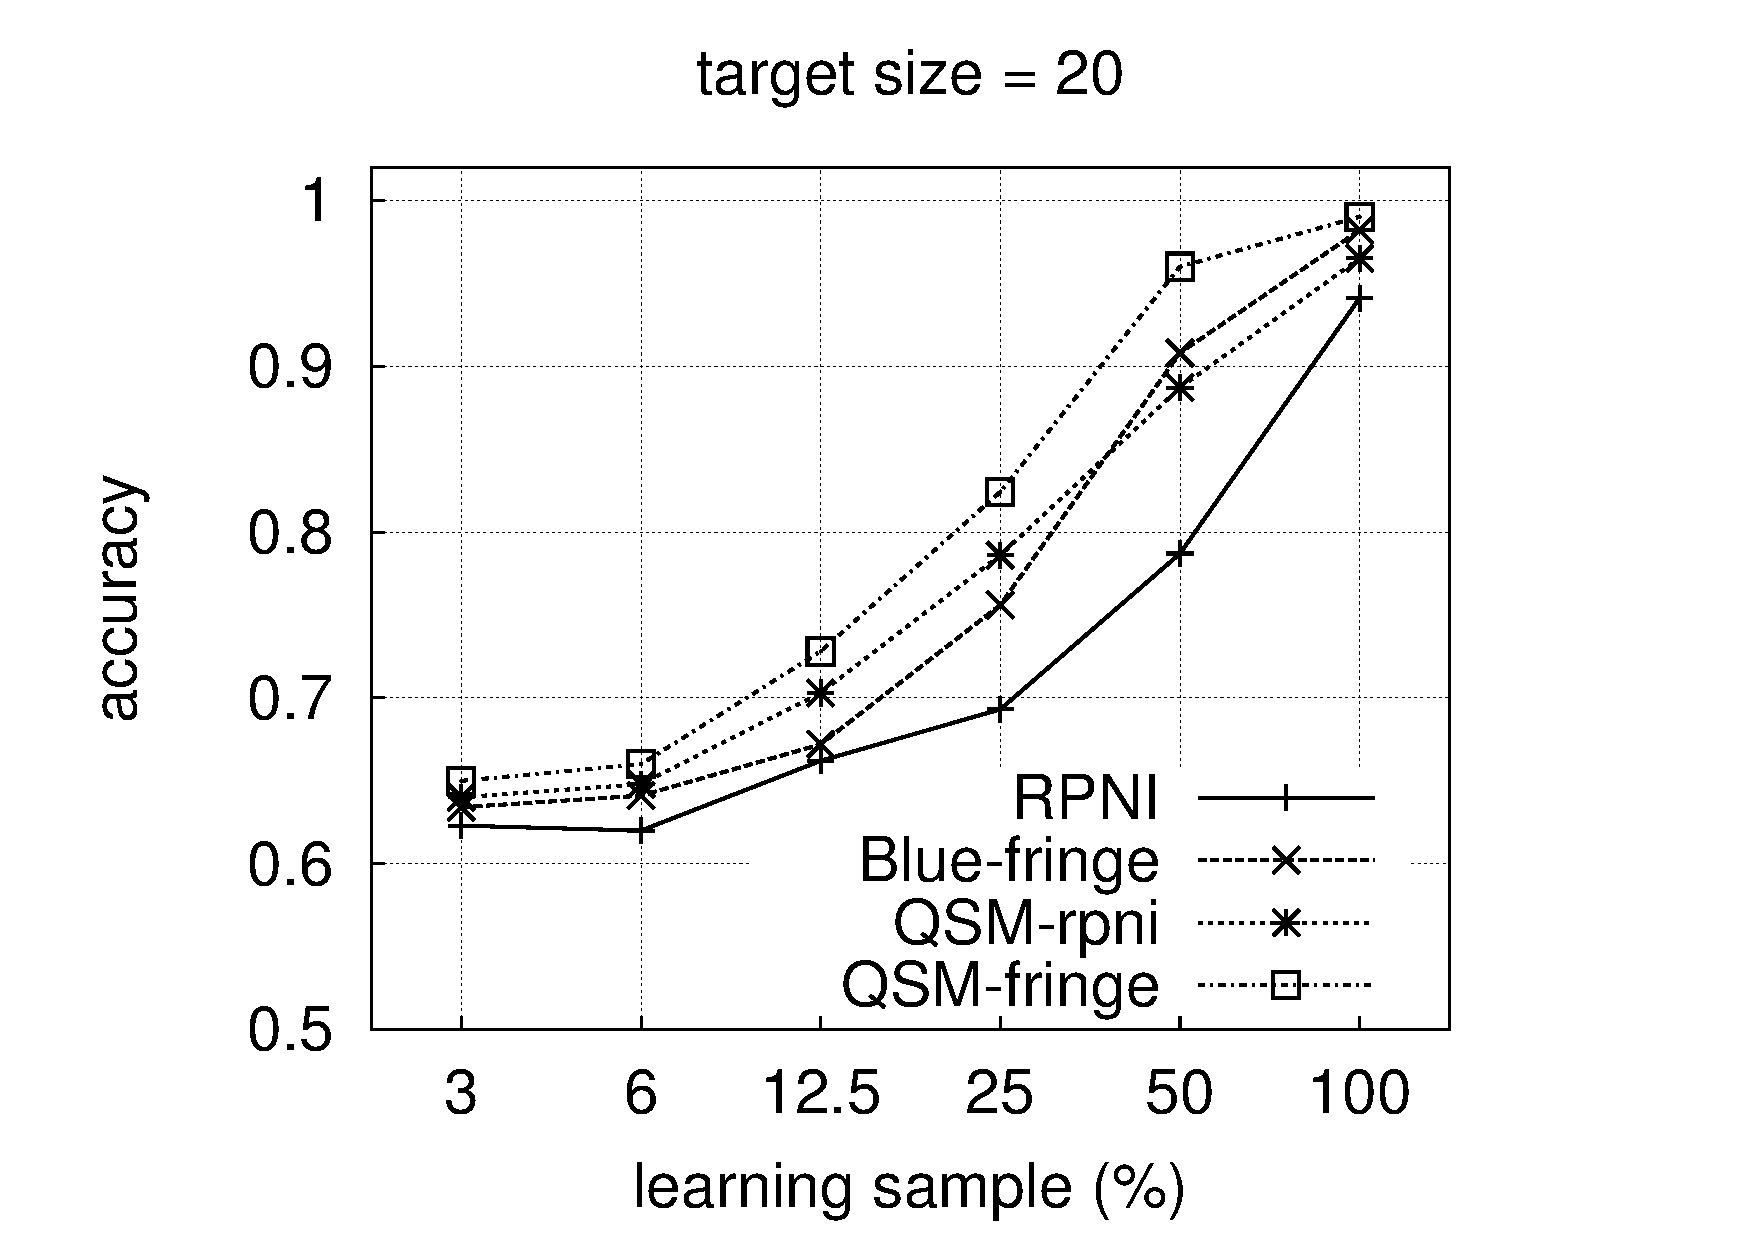
\includegraphics[trim=0mm  21mm 45mm 0mm, clip, page=1]{src/5-evaluation/images/accuracy}
  \includegraphics[trim=30mm 21mm 35mm 0mm, clip, page=2]{src/5-evaluation/images/accuracy}
}\vspace{0.35cm}
\scalebox{.25}{
  \includegraphics[trim=0mm  0mm 45mm 0mm, clip, page=3]{src/5-evaluation/images/accuracy}
  \includegraphics[trim=30mm 0mm 35mm 0mm, clip, page=4]{src/5-evaluation/images/accuracy}
}
\caption{Classification accuracy of QSM\label{image:evaluation-qsm-accuracy}.}
\end{figure}

Results from Section \ref{subsection:evaluation-bluefringe-on-casestudies} are confirmed here; Blue-fringe (resp. QSM-fringe) outperforms RPNI (resp. QSM-rpni) for sparse training samples. Moreover, significant improvements in generalization accuracy is observed thanks to the interactive feature.
\begin{itemize}
\item The QSM algorithm outperforms the original RPNI and Blue-fringe systematically.
\item Interestingly, QSM-rpni also overcomes the original Blue-fringe algorithm. In terms of model accuracy and for a fixed learning sample size, the interactive feature of QSM is at least as powerful as the evidence-driven heuristic search of Blue-fringe.
\end{itemize}

Observe that the learning sample sizes were well chosen to illustrate the convergence of this family of induction algorithms:
\begin{itemize}
\item For a given target size, the curves show the different induction phases. When the sample is sparse, 3\% or 6\% for example, poor accuracy results are first observed. The accuracy grows while the learning sample becomes larger; it does so rapidely until an accuracy of about 0.95 is reached. Beyond this point, the accuracy continues to grow with the learning sample size but much slowly. 
\item The relative performance data described above do not depend much on the target size. The curves seem successively shifted left when the target size grows. This can be explained by the fact that a quadratic learning sample in the size of the target LTS tends to be richer for large LTS than for smaller ones. 
\end{itemize}

\subsubsection*{Number of scenario questions\label{subsection:evaluation-synthetic-queries-on-qsm}}

The number of scenario questions generated to the oracle is an important feature of QSM. When the oracle is an end-user, this factor heavily impacts on the practical usability of the approach. 

Figure~\ref{image:evaluation-qsm-number-of-questions} shows the number of generated questions depending on the learning sample size, for several target sizes. The results are given for QSM-rpni and QSM-fringe. In each case, the number of generated scenarios classified by the oracle either as positive or negative are reported separately.
\begin{itemize}
\item The number of strings classified as positive tends to increase initially with the learning sample size before staying roughly constant when the learning process has nearly converged. The additional information required to guarantee correct identification mostly depends on the negative strings.
\item QSM-fringe tends to generate fewer strings classified as negative by the oracle than QSM-rpni. In both cases, however, the number of rejected queries decreases with the learning sample size. As a comparison of Fig.~\ref{image:evaluation-qsm-number-of-questions} and Fig~\ref{image:evaluation-qsm-accuracy} shows, it even reaches zero when the algorithm has converged to the exact model.
\end{itemize}

\begin{figure}
\centering
\scalebox{.25}{
  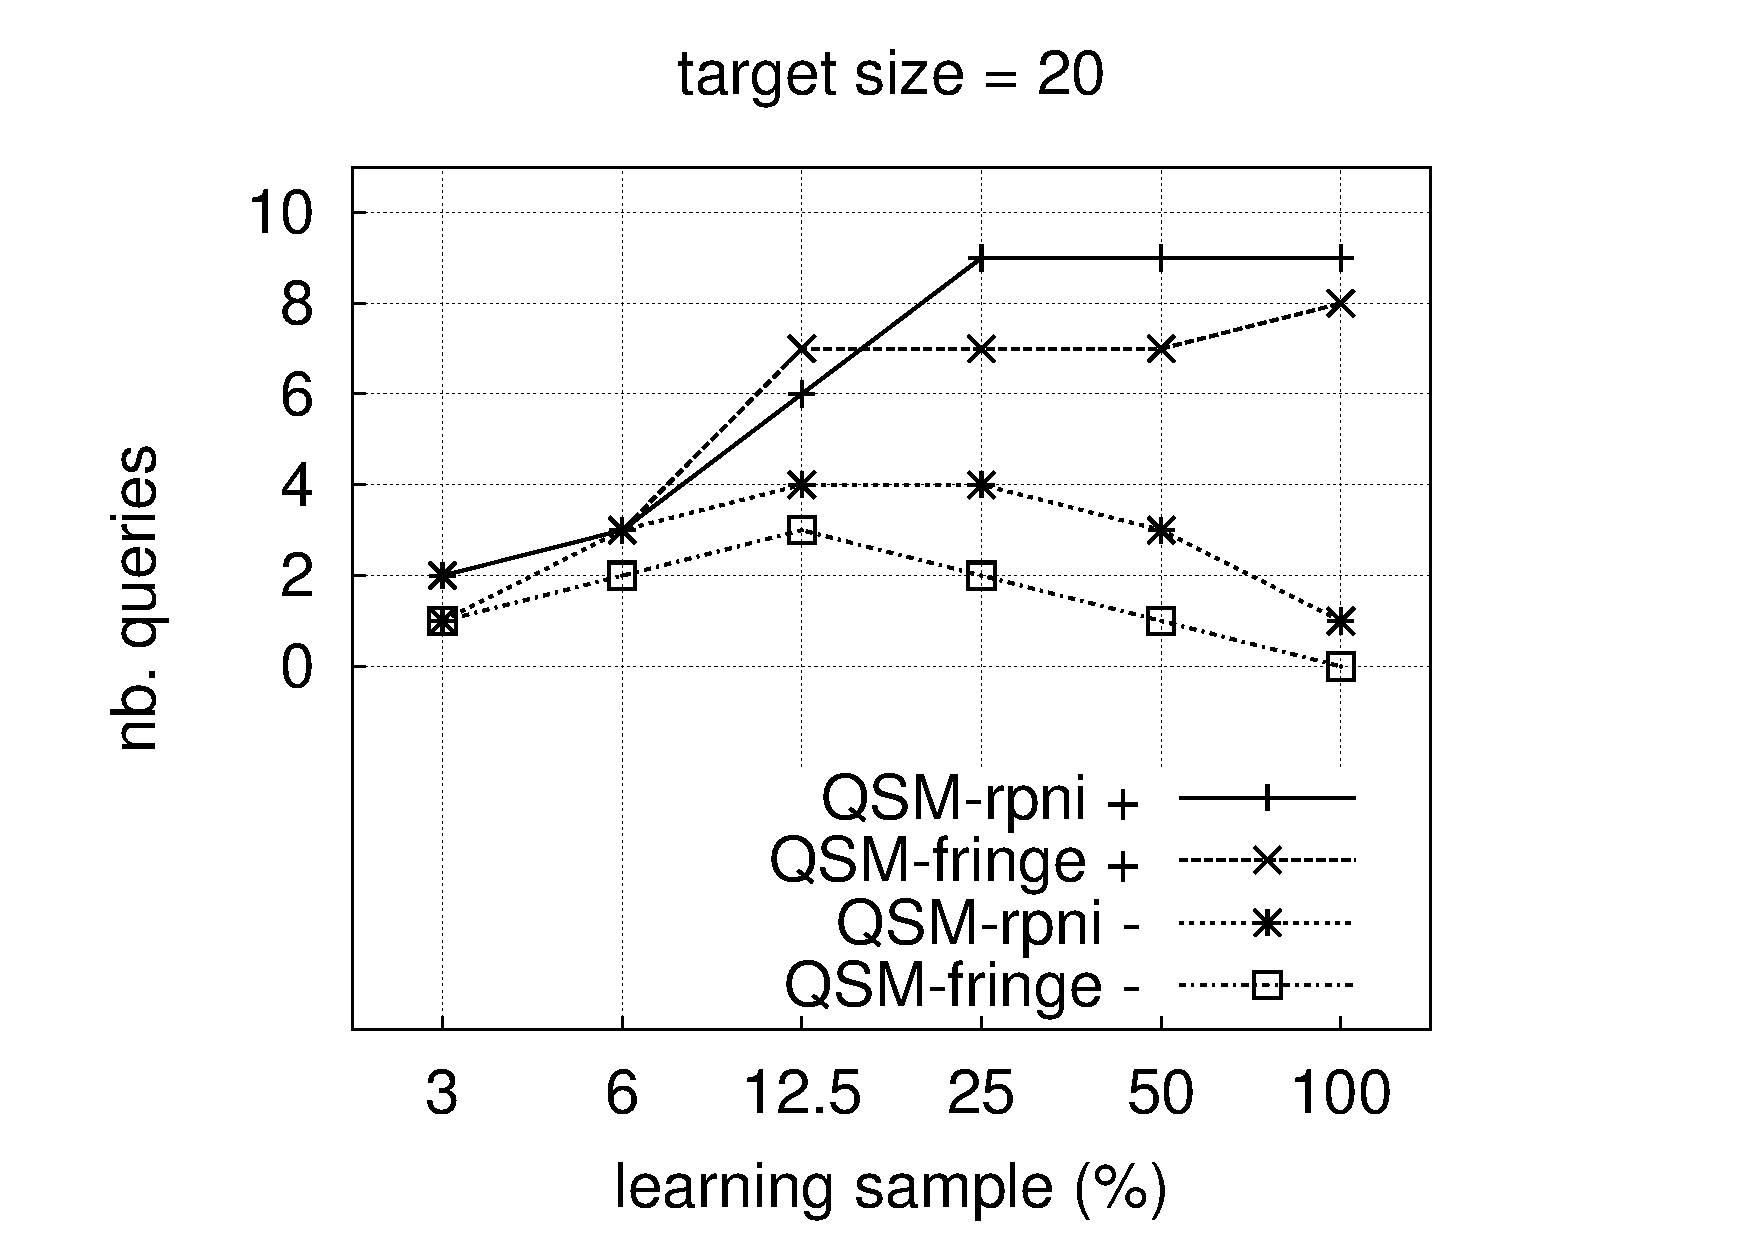
\includegraphics[trim=0mm  21mm 45mm 0mm, clip, page=1]{src/5-evaluation/images/queries}
  \includegraphics[trim=30mm 21mm 35mm 0mm, clip, page=2]{src/5-evaluation/images/queries}
}\vspace{0.35cm}
\scalebox{.25}{
  \includegraphics[trim=0mm  0mm 45mm 0mm, clip, page=3]{src/5-evaluation/images/queries}
  \includegraphics[trim=30mm 0mm 35mm 0mm, clip, page=4]{src/5-evaluation/images/queries}
}
\caption{Number of scenario questions generated by QSM\label{image:evaluation-qsm-number-of-questions}.}
\end{figure}

\subsubsection*{Induction time\label{cpu:time}}

Figure~\ref{image:evaluation-qsm-time} shows the induction time for varying learning sample size and target size. All tests were executed with Java 5.0 on a Pentium-IV 3 GHz computer with 1Gb of RAM. 

As seen there, the RPNI, Blue-fringe and QSM algorithms go through different phases according to the amount of data available:
\begin{itemize} 
\item Initially, CPU time tends to increase with the learning sample size. In this first phase, the learning time follows the increase of the sample size. 
\item When the learning sample becomes richer, better generalizations can be obtained by merging states in a more sound way. A comparison between curves in Fig.~\ref{image:evaluation-qsm-accuracy} and Fig.~\ref{image:evaluation-qsm-time} reveals that the classification rates of new data increases while the learning time is reaching its maximum. 
\item The last phase is observed when the algorithm rapidly converges to a good model. Classification accuracy tends towards 100\% while CPU time is decreased because the right merging operations are performed directly. 
\end{itemize}

\begin{figure}[t]
\centering
\scalebox{.25}{
  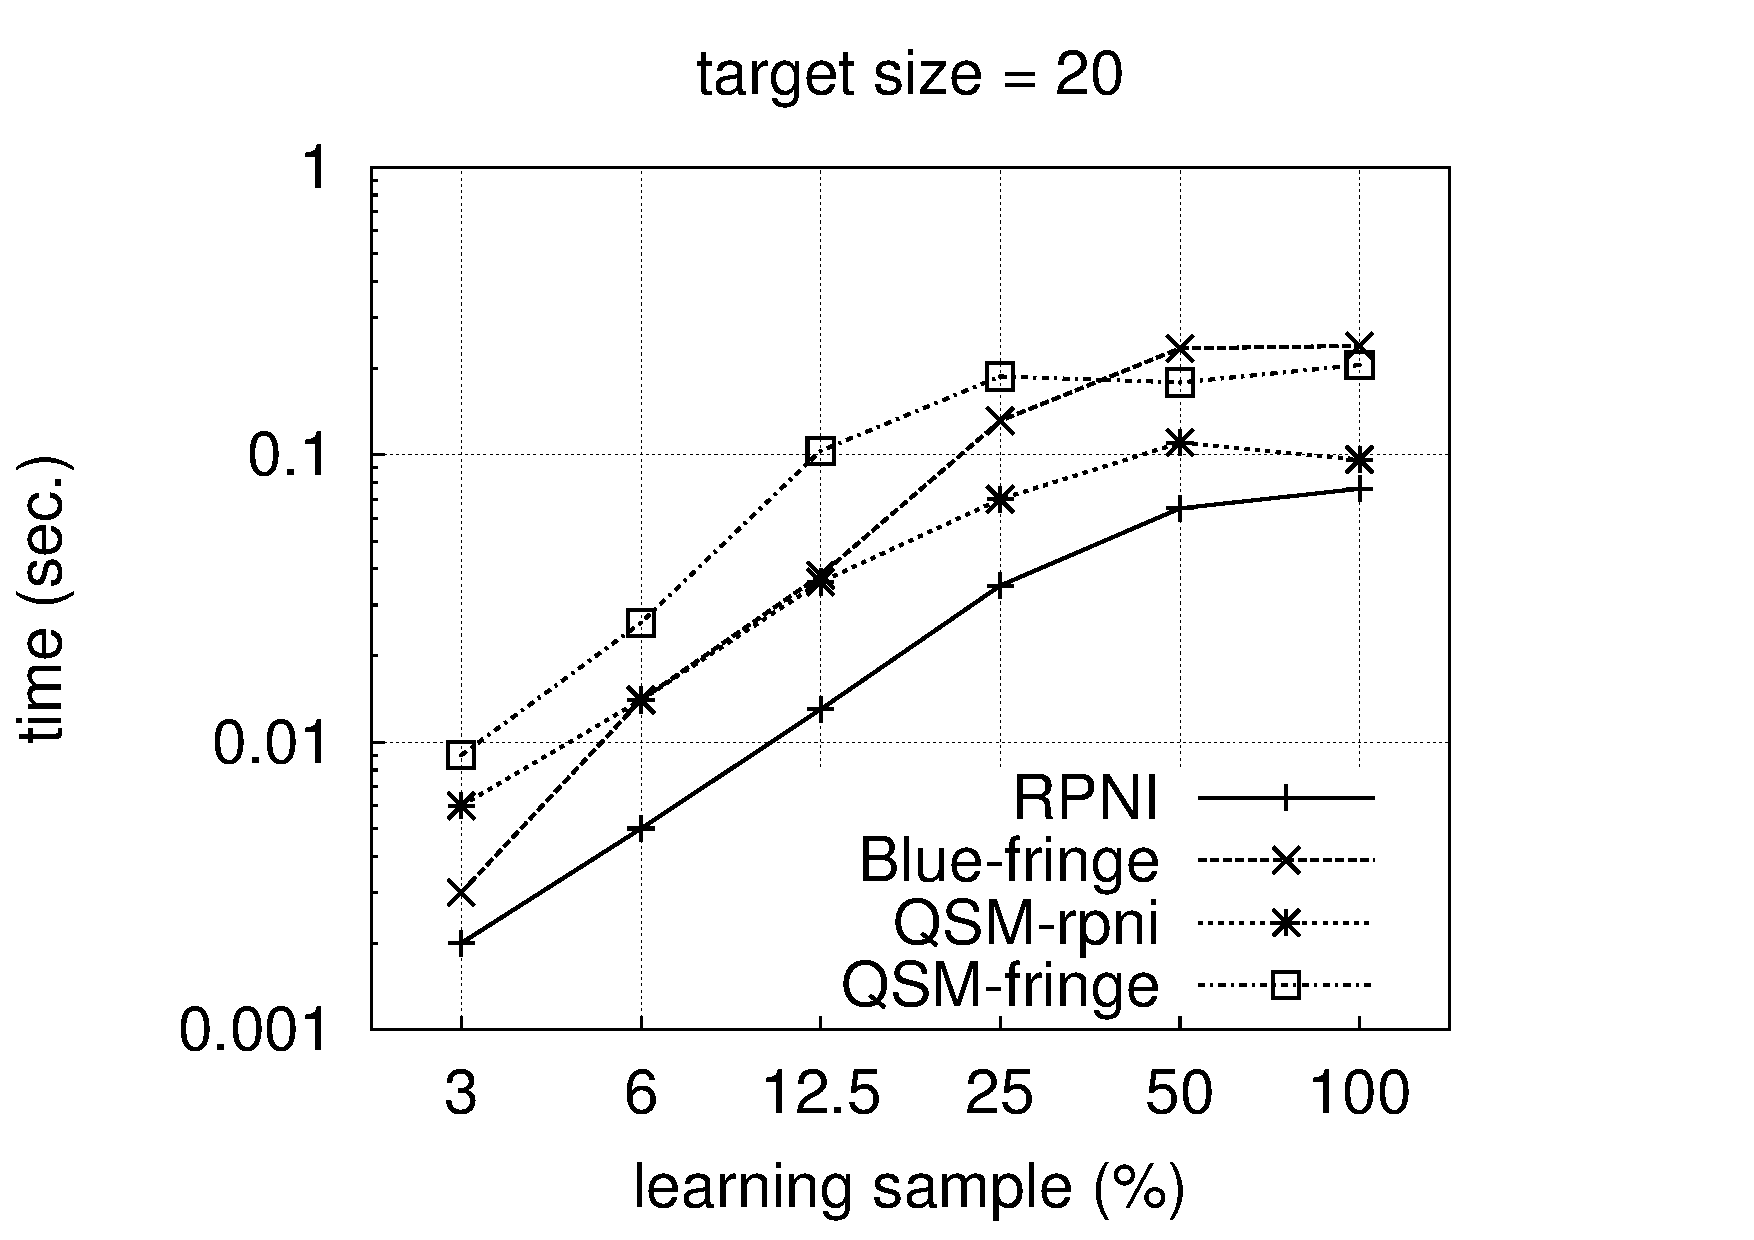
\includegraphics[trim=0mm  21mm 45mm 0mm, clip, page=1]{src/5-evaluation/images/time}
  \includegraphics[trim=30mm 21mm 35mm 0mm, clip, page=2]{src/5-evaluation/images/time}
}\vspace{0.35cm}
\scalebox{.25}{
  \includegraphics[trim=0mm  0mm 45mm 0mm, clip, page=3]{src/5-evaluation/images/time}
  \includegraphics[trim=30mm 0mm 35mm 0mm, clip, page=4]{src/5-evaluation/images/time}
}
\caption{Induction time with QSM\label{image:evaluation-qsm-time}.}
\end{figure}

The known tendencies of induction algorithms in the RPNI family were confirmed by our experiments (see, e.g., \cite{Lang:1998}). However, the curves of QSM are shifted left with respect to the learning sample size. As already observed in Fig.~\ref{image:evaluation-qsm-accuracy}, convergence is indeed faster for the QSM algorithm in that it occurs on sparser samples than RPNI or Blue-fringe. Compared to these, the relative time performance of the QSM algorithm actually depends on two contradictory effects:
\begin{itemize}
\item On the one hand, whenever a string is classified as negative by the oracle, QSM is called recursively on an extended sample. Each new call increases CPU time; such call could be considered as a new run of the RPNI or Blue-fringe algorithm. This run can however be interrupted and replaced by another one if a new negative example is included after an additional query.
\item On the other hand, due to its faster convergence QSM can obtain better results with fewer data originally provided. 
\end{itemize}
 
CPU times should thus be compared while considering the relative classification results of the various approaches. For instance, when the target size is 200 and 3\% of the full training sample is used, QSM-fringe runs an order of magnitude slower than Blue-fringe. However, the classification accuracy of QSM-fringe is 95\% while it is 67\% for Blue-fringe for the same amount of data. When the training size increases, QSM-fringe actually becomes slightly faster than Blue-fringe because it has already nearly converged to the optimal solution.

\subsection{Evaluation of ASM on synthetic datasets\label{subsection:evaluation-synthetic-asm}}

The evaluation of ASM on synthetic data is very similar to the one conducted on case studies in Section \ref{subsection:evaluation-casestudies-asm}. The objective is to quantify the gain in generalization accuracy that can be expected when the proportion of domain-specific control information \`a la hMSC is increased as input. 

The experimentation protocol used to achieve this objective is a slight adaptation of the one discussed in Section \ref{subsection:evaluation-synthetic-protocol}.
\begin{itemize}
\item Experiments here were made on randomly generated target LTS with 32 and 64 states. Following Abbadingo, alphabets still had two symbols only (we further discuss this limitation in Chapter~\ref{chapter:stamina}).
\item Learning and test samples were randomly generated as before. RPNI and Blue-fringe were both evaluated on these samples to provide a reference for the comparisons with ASM.  
\item In order to provide its input to ASM, a specific procedure simulated the control information given by a hMSC:
\begin{itemize}
\item For a given learning sample, an augmented PTA was first built. As in Section \ref{subsection:evaluation-casestudies-asm}, an early state merging phase then occured. The idea was to merge specific state pairs of the PTA that were known to correspond to the same state in the target LTS.
\item For this, unique labels were associated to randomly chosen states of the target LTS. Increasing proportions of the number of states labeled in this way were used, namely, 5\%, 10\%, 20\% and 100\%. The PTA and the target LTS are were then jointly visited and state labels are reported as decorations of the PTA states. 
\item States of the PTA sharing the same label were merged early. This effectively simulated the availability of control information through a hMSC by introducing loops in the input scenarios. The automaton resulting from this step was then used as input of ASM, that further generalized it by merging additional state pairs under the control of the negative strings.
\end{itemize}
\end{itemize}
 
Figure~\ref{image:evaluation-asm-accuracy} reports the proportion of independent test samples correctly classified while increasing the learning sample. Curves in these plots correspond to executions of RPNI, Blue-fringe and ASM with different labeling proportions. Each point in these plots represents the average value computed over 200 independent runs. 

\begin{figure}
\begin{center}
\scalebox{.28}{\includegraphics*{src/5-evaluation/images/asm-accuracy.jpg}}
\caption{Classification accuracy for ASM\label{image:evaluation-asm-accuracy}.}
\end{center}
\end{figure}

ASM overcomes RPNI on all executions, which is actually expected. Remember from Section~\ref{subsection:automaton-state-merging} that ASM reduces to RPNI in the special case where its input is a PTA, that is, when no early state merging occurs in our experiment. By construction of our experiment, the early state merging performed are sound. Therefore, they could not hurt the generalization accuracy; hence, ASM can only produce the same or a better accuracy score than RPNI.

From the standpoint of generalization accuracy, however, 5\% of the labeling information is comparable to the use of the Blue-fringe heuristic for selecting state pairs to be merged. Beyond this proportion, the accuracy keeps increasing. Interestingly, the accuracy gain is already visible when the sample is sparse.

Note that the identification of the target does not reduce to a trivial problem even with 100\% of labeling information. As discussed in Section \ref{section:inductive-from-hMSC}, control information is complementary but does not substitute to the negative knowledge provided by negative scenarios, fluent and goals. In particular, it does not prevent overgeneralization from occuring when incompatible state pairs are merged. 

\section{Summary and discussion\label{section:evaluation-summary}}

This chapter discussed the evaluation of the inductive LTS synthesis technique presented in Chapter \ref{chapter:inductive-synthesis}. Evaluations have been conducted on case-studies and complemented with experiments on synthetic datasets. The latter provide an overview of what can be expected along two dimensions not completely covered with case-studies: the size of the target LTS model and the sparsity of the learning sample.  

From the point of view of multi-view model synthesis, the following conclusions can be drawn:
\begin{itemize}

\item Together with the Blue-fringe heuristics, the interactive feature of QSM is very effective for reaching a good accuracy of synthesized models. The cost in terms of scenario questions may be important, especially on large systems. Therefore, techniques to reduce the number of scenarios to be classified are required in practice.

\item Among our pruning techniques, the domain knowledge provided by fluents, goals and legacy components proves very useful. In addition to reducing the number of scenario questions, such knowledge effectively guides the induction process toward accurate LTS models. 

\item The control information given by a hMSC, simulated in evaluations through a dedicated procedure, also provides an important accuracy gain. While it guides the generalization process toward good generalizations, it has been shown that it does not provide the negative knowledge required to avoid over-generalization.

\item The most important issue with QSM is related to the number of generated scenario questions. As shown in Table~\ref{All:res} and in Fig.~\ref{image:evaluation-qsm-number-of-questions}, the number of rejected questions tend to decrease when the induction input gets richer, either because the sample gets larger or thanks to available domain knowledge. The same is not true for scenarios to be accepted, whose number gets roughly constant.

In practice, this means that QSM will generate scenarios even when its input is rich enough to guarantee very good generalizations without even asking questions (e.g., when given a characteristic sample). Moreover, fluents and goals do not help reducing these questions. As their number might become large for non-toy systems, improvements of our technique might be necessary.

One possible solution could be to extend the possible answers from the oracle. For example, the end-user could request to terminate the induction immediately, without additional scenario questions. The infered state machine would then be submitted for inspection, leading to a form of \emph{equivalence} queries. Such queries are typically answered with an additional negative scenario and the induction restarted if the state machine is not adequate (e.g. \cite{Angluin:1987}, see also Chapter~\ref{chapter:discussion}).

\end{itemize}

We close this chapter by discussing specific issues related to the experiments themselves and the protocols used to conduct them. 
\begin{itemize}

\item The coverage of conducted experiments could be slightly extended. In particular, the use of control information and ASM could be further studied with more case-studies. The real use of a hMSC instead of a simulation procedure is worth considering as well.

Our current implementation of ASM relies on the RPNI search order and does not support the interactive feature of QSM. This limited the possible comparisons during evaluations. In particular, the effect of control information on the number of generated questions has not been illustrated.

\item The experiments on synthetic datasets provide an in-depth analysis of the performances of QSM and ASM with RPNI and Blue-fringe, which have been taken as state-of-the-art induction algorithms. 

Another induction algorithm called DFASAT recently appeared that significantly outperforms RPNI and Blue-fringe \cite{Heule:2010} (see Chapter~\ref{chapter:stamina}). This opens new perspectives for comparisons, evaluations and further developments around QSM and ASM. 

\item In contrast to the smaller but ``real'' case studies, the experiments on synthetic datasets are such that target LTS are defined on alphabets of two symbols only. This is a consequence of reusing the protocol from Abbadingo for conducting experiments. 

As shown by the case studies themselves, state machines of software systems are commonly defined on larger alphabets. While this does not hurt the soundness of our experiments themselves, it slighlty prevent from generalizing their results. The next chapter addresses this issue by describing our work on the Stamina plateform for evaluating inductive model synthesis techniques with an alternative protocol to Abbadingo.
\end{itemize}

